\documentclass[aspectratio=43]{beamer}

\usepackage[french]{babel}
\usepackage{caption}
\usepackage[T1]{fontenc}
\usepackage{amsmath, amsfonts, amssymb, mathtools}
\usepackage{stmaryrd}
\usepackage{fancyhdr}
\usepackage{lipsum}
\usepackage{graphicx}
\usepackage[ddmmyyyy]{datetime}
\usepackage{adjustbox}
\usepackage[explicit]{titlesec}
\usepackage{pdfpages}
\usepackage{tikz}
\usepackage{pifont}
\usepackage{fontawesome5}
\usepackage{algpseudocode}
\usepackage{algorithm2e}

\usetheme{Boadilla}

\definecolor{white}{gray}{0.98}
\definecolor{green}{HTML}{92D050}
\usefonttheme[onlymath]{serif}

\makeatletter
\definecolor{beamer@darkblue}{HTML}{000065} % changed this
\setbeamertemplate{frametitle}{\color{beamer@darkblue}\bfseries\insertframetitle\par\vskip-6pt\hrulefill}

\graphicspath{{./img/}}

\title[Automates Cellulaires]{TIPE - Automates cellullaires continus}
\subtitle{Et leurs applications \`a la mod\'elisation de vie artificielle}
\author{Ars\`ene MALLET}
\date[\today]{\today}
\institute{Candidat - 22669}

\begin{document}


\begin{frame}
	\titlepage
\end{frame}

\begin{frame}
	\frametitle{Introduction}

	\begin{itemize}
		\setlength\itemsep{2em}
		\item Jeu a z\'ero-joueur : d\'etermin\'e par les
			conditions initiales
		\item "Jeu de la vie" par John Conway $\rightarrow$ espace \textbf{discret}
		\item G\'en\'eralisation dans l'espace \textbf{continu} $\rightarrow$ \textbf{Lenia}
	\end{itemize}
\end{frame}

\begin{frame}
	\frametitle{Convolution}

	\begin{block}{Produit de convolution :}
		Si $f, g$ deux fonctions réelles ou complexes, $$ (f \star g)(x) = \int_{-\infty}^{+\infty} f(x-t)g(t)\,dt$$

		Espace discret, si $f, g$ définies sur $\mathbb{Z}$, alors
		$$ (f \star g)[n] = \sum_{m = -\infty}^{+\infty} f[m]g[n - m]$$
	\end{block}

	\begin{block}{Noyau de convolution - Filtre :}
		Une fonction réelle ou complexe $\mathbf{K}$ dont on fait le produit de convolution
		avec une autre fonction.
	\end{block}
\end{frame}

\begin{frame}
	\frametitle{Automate Celullaire}

	\begin{block}{Automate Cellulaire :}
		Un automate cellullaire $\mathcal{A}$ est caract\'eris\'e par un 5-uplet
		$(\mathcal{L}, \mathcal{T}, \mathcal{S}, \mathcal{N}, \phi)$ où :
		\begin{itemize}
			\item $\mathcal{L}$ est un espace euclidien
			\item $\mathcal{T}$ est la "chronologie", ou la dimension temporelle de l'automate (suite : $\mathcal{T} = \mathbb{R}_+$)
			\item $\mathcal{S}$ est l'ensemble des états de l'automate
			\item $\mathcal{N} \subset \mathcal{L}$ est le voisinage de l'origine
			\item $\phi : \mathcal{S}^{\mathcal{N}} \rightarrow \mathcal{S}$ est la règle locale d'évolution
		\end{itemize}
	\end{block}


\end{frame}

\begin{frame}
	\frametitle{Jeu de la Vie (GoL)}

	\textbf{Jeu de la vie} $\longrightarrow$ $(\mathbb{Z}^2, \{0, 1\}, \{-1, 0, 1\}^2, \phi)$ o\`u
	\[
		\phi(x) = 
		\begin{cases}	
			1 \text{ si } x = 1, \mathcal{N}_x \in \{2, 3\} \text{ (survie)} \\
			1 \text{ si } x = 0, \mathcal{N}_x = 3 \text{ (naissance)} \\
			0 \text{ sinon (mort)}
		\end{cases}
	\]

	\centering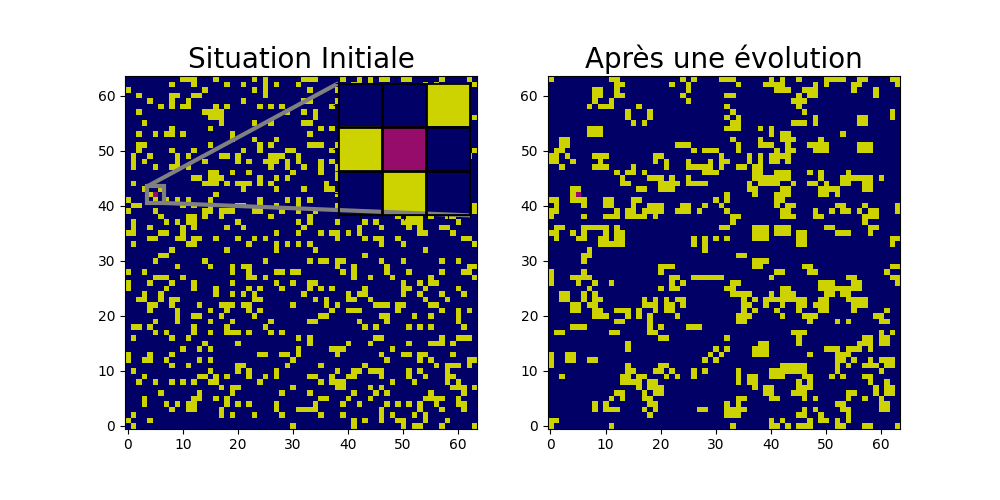
\includegraphics[width=.9\textwidth]{plot_evolution_gol.png}
	
\end{frame}

\begin{frame}
	\frametitle{Formes de vie}
	\centering
	Forme de vie $\approx$ \textbf{Comportement(s) "remarquable(s)"}

	\vspace{20pt}
	Exemples dans GoL (\textbf{survie stationnaire : "block", oscillateur : "blinker", d\'eplacement : "glider"}):

	\centering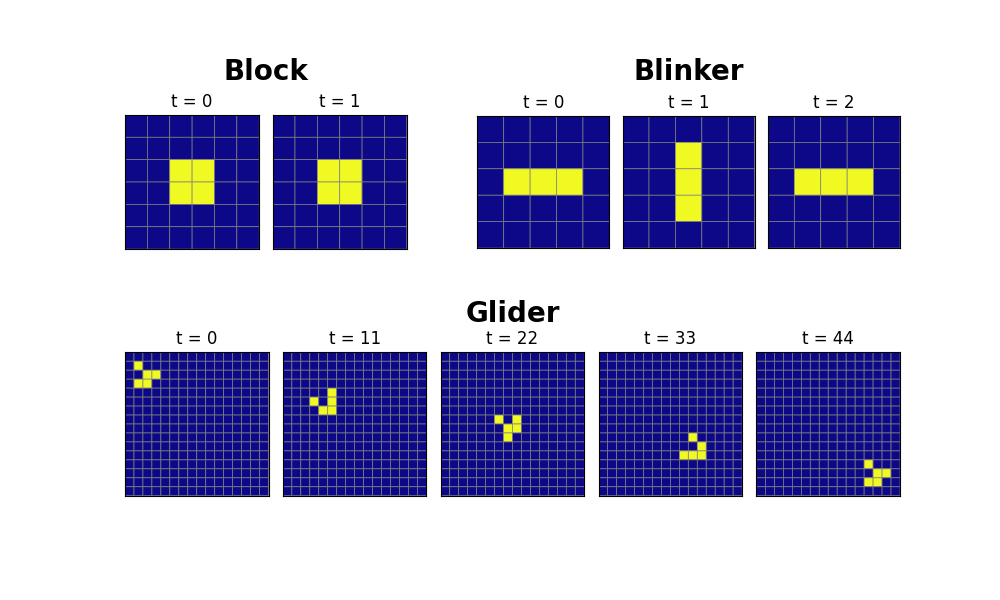
\includegraphics[width=.9\textwidth]{plot_species_gol.png}

\end{frame}

\begin{frame}
	\frametitle{Lenia (1)}

	\begin{block}{Configuration :}
		On définit $\mathbf{A}^t : \mathcal{L} \rightarrow \mathcal{S}$ comme la \textit{configuration}
		ou \textit{collection d'etats} dans l'espace à un instant $t \in \mathcal{T}$.

		Ainsi, $ \forall t \in \mathcal{T}, \forall x \in \mathcal{L}, \mathbf{A}^t(x)$ est l'état de $x$
		à l'instant $t$.
	\end{block}
	
	L'automate cellulaire Lenia est d\'efini par :
	\begin{itemize}
		\item $\mathcal{L} = \mathbb{R}^2$
		\item $\mathcal{S} = [0, 1]$
		\item $\mathcal{N} = \mathbf{B}_{\lVert \cdot \rVert_2}(0, 1)$
		\item $\phi = \operatorname{Id} + dt \cdot \mathbf{G} \circ \mathbf{U}$, o\`u  $\mathbf{G} : [0, 1] \mapsto [-1, 1] $, \textbf{fonction de croissance} et $\mathbf{U} : \mathcal{S}^\mathcal{N} \mapsto [0, 1]$, \textbf{distribution de "potentiel"}.
	\end{itemize}
\end{frame}

\begin{frame}
	\frametitle{Lenia (2)}

	\begin{alertblock}{\'Etape d'\'evolution}
		\begin{itemize}
			\item Pour tout point $x \in \mathcal{L}$, on calcule son "potentiel" : $$\mathbf{U}^t(x) = \mathbf{K} \star \mathbf{A}^t(\mathcal{N}_x)$$
			\item On met ensuite la configuration à jour :
				\begin{align*}
					\forall x \in \mathcal{L}, \mathbf{A}^{t + dt}(x) &= \phi(\mathbf{A}^{t}(\mathcal{N}_x)) \\
					&= \mathbf{A}^t(x) + dt \cdot \mathbf{G}(\mathbf{U}^t(x))
				\end{align*}
			\item On tronque les \'eventuelles valeurs qui ne sont pas dans $[0, 1]$
		\end{itemize}
	\end{alertblock}
\end{frame}

\begin{frame}
	\frametitle{Lenia (3)}

	\begin{columns}
		\begin{column}{0.5\textwidth}
			Exemples de noyaux de convolution :
			\[
				\mathbf{K}(r) = 
				\begin{cases}	
					\exp\left(-\displaystyle\frac{(r - \gamma)^2}{2\delta^2}\right) ; \gamma, \delta \in \mathbb{R} \\
					4r^\alpha(1-r)^\alpha ; \alpha \in \mathbb{N}^* \\
					\mathbf{1}_{[a, b]}(r)
				\end{cases}
			\]
		\end{column}
		\begin{column}{0.5\textwidth}
			\begin{center}
				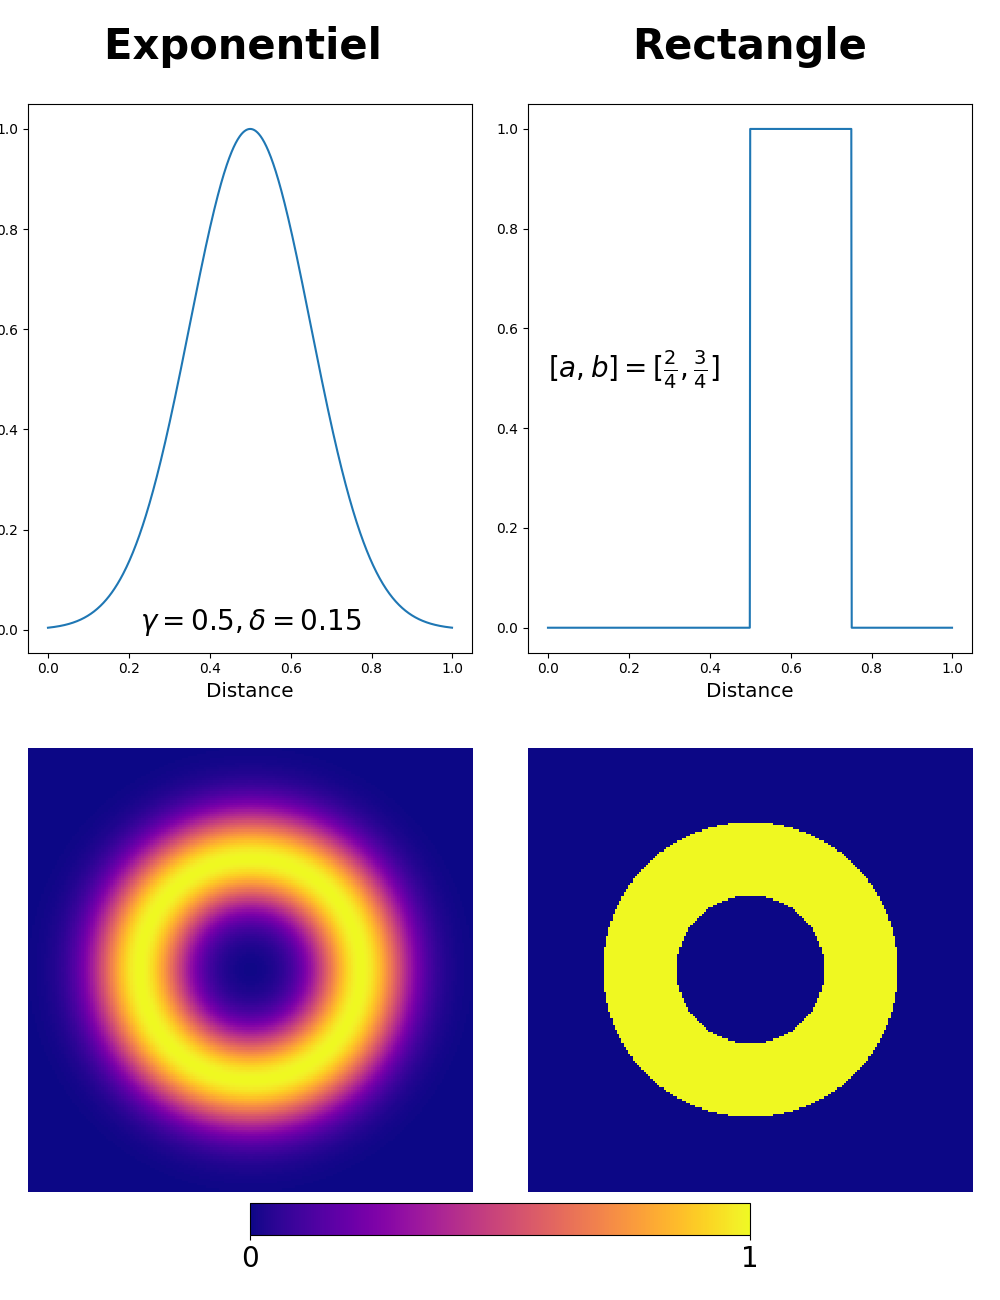
\includegraphics[width=0.9\textwidth]{plot_convolution_kernels.png}
			\end{center}
		\end{column}
	\end{columns}

\end{frame}

\begin{frame}
	\frametitle{Lenia(3)}
	Exemples de fonctions de croissance:
	\[
		\mathbf{G}(u) = 
		\begin{cases}	
			2\exp\left(-\displaystyle\frac{(u - \mu)^2}{2\sigma^2}\right) - 1 & \mu, \sigma \in \mathbb{R} \\
			2\mathbf{1}_{[\mu \pm \sigma]}(u) - 1 & \mu, \sigma \in \mathbb{R} \\
		\end{cases}
	\]
	\begin{center}
		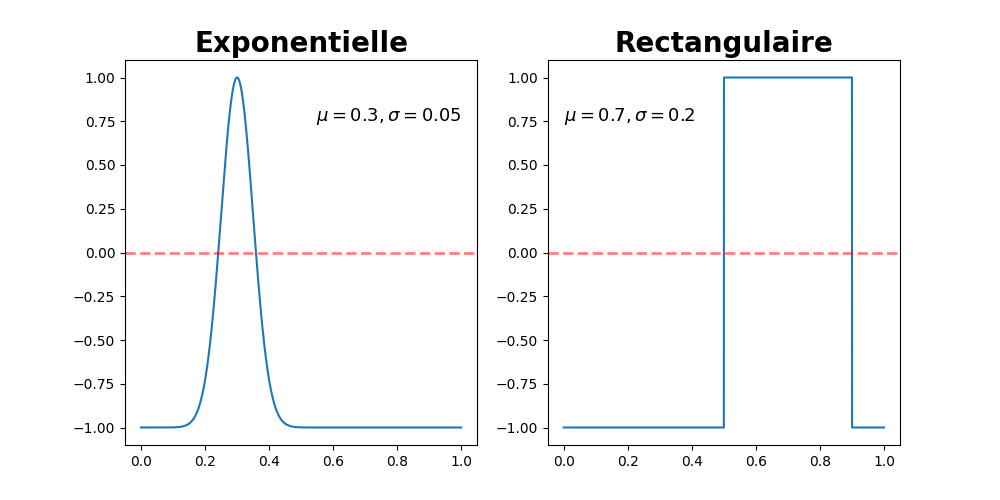
\includegraphics[width=0.9\textwidth]{plot_growth_mapping.png}
	\end{center}
\end{frame}

\begin{frame}
	\frametitle{Exemple d'evolution}

	\centering

	\textbf{Conditions initiales} : Grille remplie \textbf{al\'eatoirement}, Noyau \textbf{exponentiel} ($\gamma = 0.5, \delta = 0.15$), croissance \textbf{exponentielle} ($\mu = 0.5, \sigma = 0.015$)

	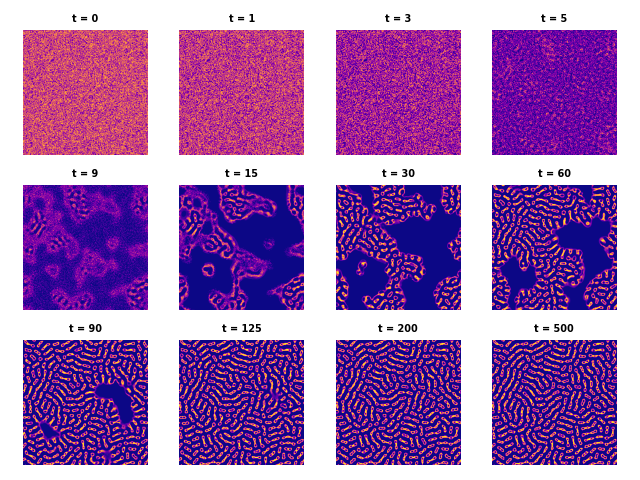
\includegraphics[height=.75\textheight]{evolution_lenia_random_init.png}

\end{frame}

\begin{frame}
	\frametitle{Exemple de perturbation}

	\centering

	\textbf{M\^eme} conditions initiales + \textbf{Perturbation \`a $t = 200$}

	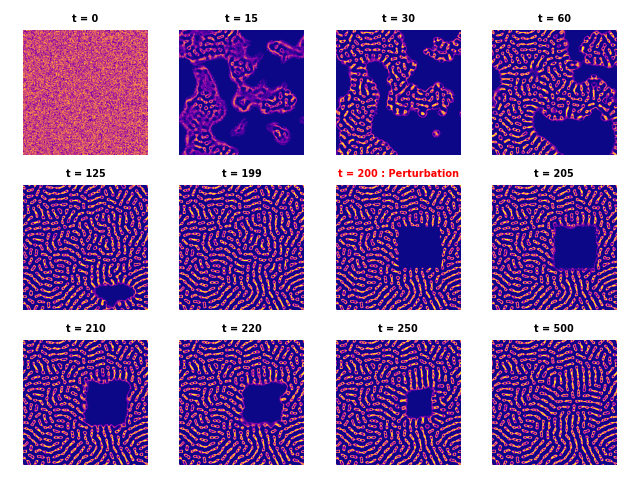
\includegraphics[width=.75\textwidth]{evolution_lenia_random_init_perturbation.png}

	Esp\`ece \textbf{stable/r\'esistante}

\end{frame}

\begin{frame}
	\frametitle{Orbium, le "glider continu"}

	\centering

	Glider (GoL) $\rightarrow$ \textbf{d\'eplacement} $\leftarrow$ Orbium (Lenia)

	\vspace{5pt}

	M\^eme noyau, m\^eme fonction de croissance, \textbf{diff\'erente grille d'initialisation}

	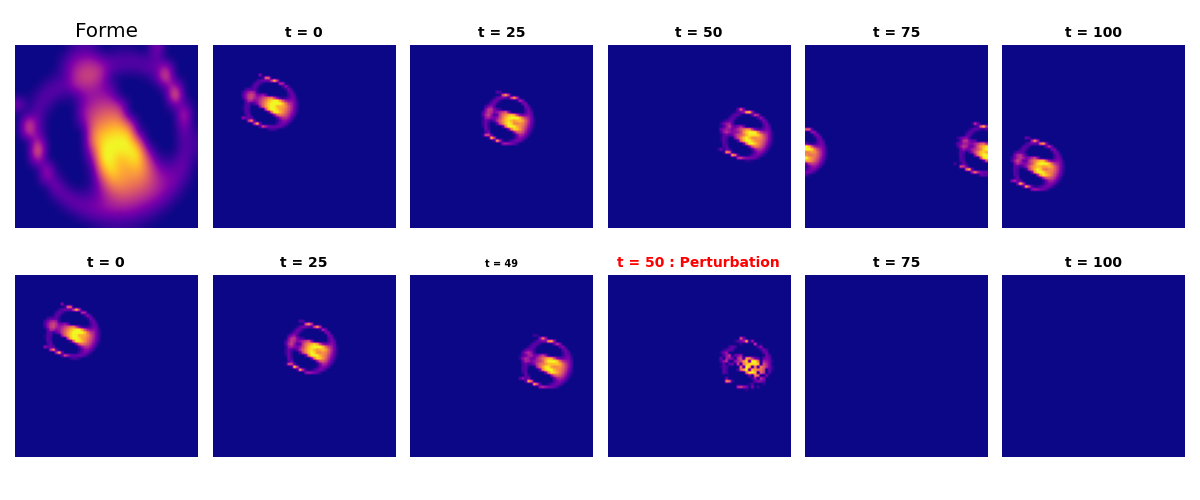
\includegraphics[width=0.85\textwidth]{evolution_orbium.png}

	Esp\`ece \textbf{non stable/r\'esistante}

\end{frame}

\begin{frame}[c]

	\centering
	\begin{Large}
		Comment \textbf{trouver} des formes de vie ?
	\end{Large} \\
	"A la main" : difficile et pas tr\`es efficace \\
	$\rightarrow$ \textbf{Apprentissage automatique}

	\vfill

	\begin{Large}
		Comment les rendre \textbf{r\'esistantes} ?
	\end{Large} \\
	$\rightarrow$ Ajout de \textbf{perturbations durant l'entra\^inement}

	\vfill

	\begin{Large}
		 Peuvent-elles s'\textbf{adapter} \`a leur environnement ?
	\end{Large} \\
	$\rightarrow$ Test avec diff\'erentes perturbations \textbf{inconnues}


\end{frame}

\begin{frame}
	\frametitle{Noyau \`a multi-anneaux}
	Multi-anneaux exponentiels, choix des amplitudes $A_i \in [0, 1]$, des distances caract\'eristiques $\gamma_i$
	et des tailles caract\'eristiques $\delta_i$.
	
	$$ K(r) = \sum_{i=0}^{N} A_i \exp\left(-\displaystyle\frac{(r - \gamma_i)^2}{2\delta_i^2}\right)$$
	
	Exemple avec $A = (0.3; 1; 0.7; 0.2); 
	\gamma = (0.2; 0.4; 0.6; 0.8);
	\delta = (0.015; 0.05; 0.01; 0.1)$

	\vspace*{5pt}

	\centering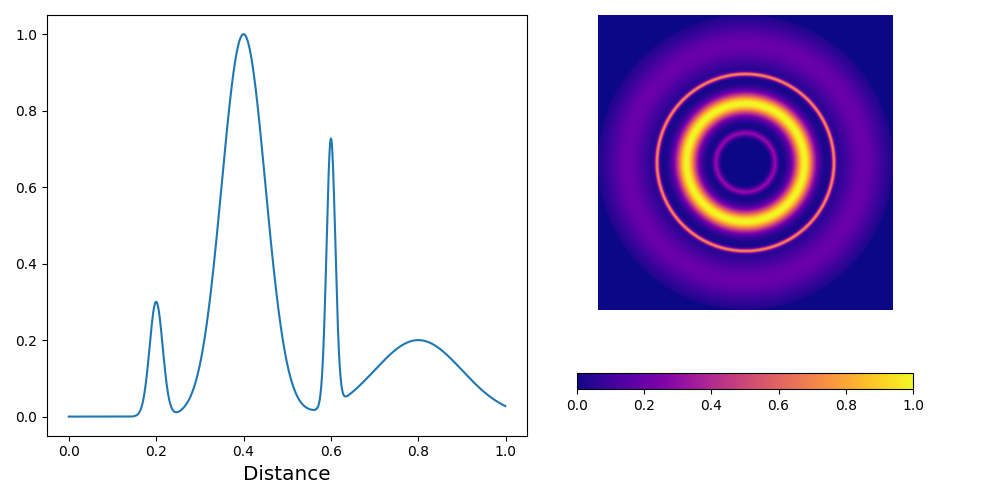
\includegraphics[width=.6\textwidth]{plot_multi_ring_kernel.png}
	
\end{frame}

\begin{frame}
	\frametitle{Exemple d'une telle esp\`ece, le Quadrium}
	\centering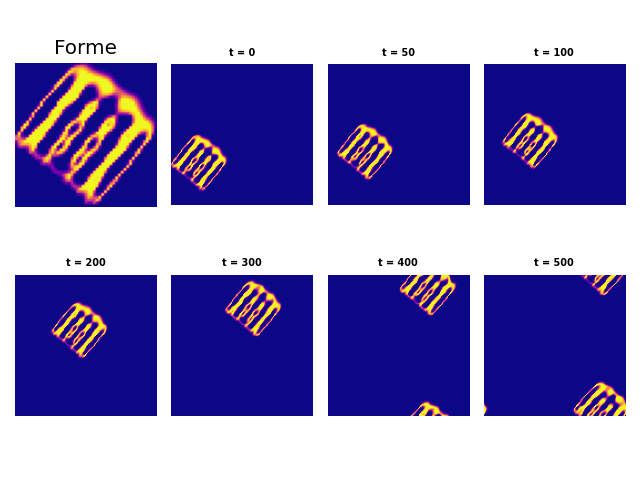
\includegraphics[width=\textwidth]{evolution_quadrium.png}
\end{frame}

\begin{frame}
	\frametitle{Les configurations multicanaux}
	
	\begin{itemize}
		\item Un \textbf{canal} est associ\'e \`a une \textbf{configuration} $\mathbf{A}_i$
		\item On consid\`ere des couples $(\mathbf{K}, \mathbf{G})_{i, s_i, d_i}$, o\`u $s_i$ est le \textbf{canal source} et $d_i$ celui \textbf{d'arriv\'ee}
		\item Pour une \'etape, si $c$ un canal :
		\[
			\mathbf{A}^{t+dt}_c(x) = \mathbf{A}^t_c(x) + dt \sum_{i ,\; d_i = c} \mathbf{G}_{i, s_i, d_i}(\mathbf{K}_{i, s_i, d_i} \star A_{s_i}^t(\mathcal{N}_x))  
		\]
	\end{itemize}
\end{frame}

\begin{frame}
	\frametitle{Une esp\`ece multicanal, le Tessellatium (1)}

	Graphique des \textbf{diff\'erents noyaux du Tessellatium} :
	
	\begin{center}
		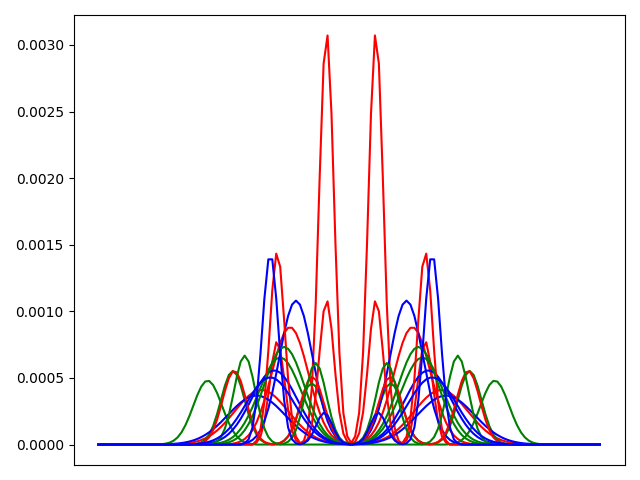
\includegraphics[width=0.7\textwidth]{plot_kernel_multi_channel.png}
	\end{center}

	\textbf{Chaque couleur} correspond \`a \textbf{un m\^eme canal}
\end{frame}

\begin{frame}
	\frametitle{Une esp\`ece multicanal, le Tessellatium (2)}

	\centering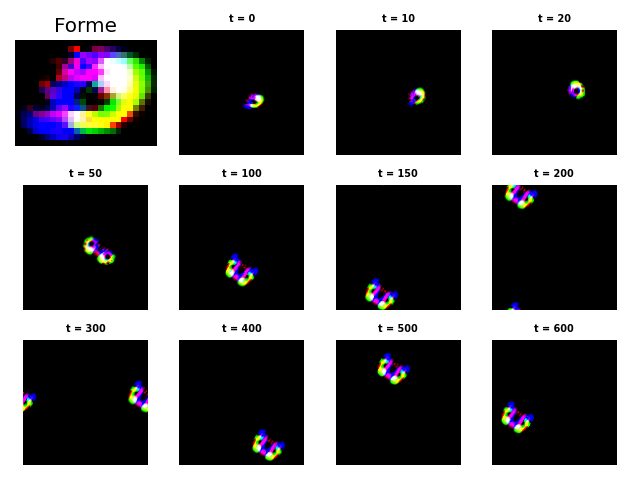
\includegraphics[width=0.9\textwidth]{evolution_aquarium.png}
\end{frame}

\begin{frame}
	\frametitle{Optimisation de la convolution}

	\begin{block}{Transformation de Fourier}
		Si $f$ est une fonction int\'egrable sur $\mathbb{R}$,
		\[
			\mathbf{F}(f) \colon \omega \mapsto \int_{-\infty}^{+\infty} f(x)e^{-i \omega x}\,dx
		\]
		Cette fonction est inversible, on note $\mathbf{F}^{-1}$ son inverse.
	\end{block}
	\begin{alertblock}{Theor\`eme de convolution}
		Si $f, g$ deux fonctions int\'egrables sur $\mathbb{R}$ alors,
		\[
			f \star g = \mathbf{F}^{-1}(\mathbf{F}(f)\mathbf{F}(g))
		\] \end{alertblock}

	Informatiquement si $A, B \in \mathcal{M}_n(\mathbb{R})$; Convolution classique : $O(n^4)$, en utilisant
	la transformation de Fourier : $O(n^2\log(n))$
\end{frame}

\begin{frame}
	\frametitle{Descente du gradient}
	But : \textbf{Minimiser} une fonction $\rightarrow$ \textbf{descente du gradient}
	\begin{alertblock}{Algorithme}
		Si $E$ un espace pr\'ehilbertien et $f : E \rightarrow \mathbb{R}$ une fonction diff\'erentiable, $\varepsilon > 0$ un seuil et $x_0 \in E$ un point de d\'epart :
		\begin{enumerate}
			\item Pour $k \in \mathbb{N}$, on calcule $\nabla f(x_k)$
			\item Si $\lVert \nabla f(x_k) \rVert \leqslant \varepsilon$, arr\^et.
			\item Sinon, on choisit un pas $\theta_k > 0$, et $$x_{k + 1} = x_k - \theta_k \nabla f(x_k)$$
		\end{enumerate}	
	\end{alertblock}
	On choisit g\'en\'eralement les $\theta_k$ par \textbf{recherche lin\'eaire}
\end{frame}
\begin{frame}
	\begin{center}
		\small\textbf{I}ntrinsically \textbf{M}otivated \textbf{G}oal \textbf{E}xploration \textbf{P}rocesses : Processus d'exploration des objectifs motivés intrinsèquement
	\end{center}
	\begin{alertblock}{Apprentissage automatique progressif (IMGEP)(1)}
		\begin{algorithm}[H]
			$n_\text{init}$ configurations al\'eatoires, stocker ($p$, $r$) dans m\'emoire $\mathbf{M}$\;
			\For{$n_\text{IMGEP}$}{
				\'Etablir un r\'esultat cible $r_t$ (pas trop loin de ceux dans $\mathbf{M}$)\;
				Chercher dans $\mathbf{M}$, les param\`etres $p$ donnant le résultat le + proche la cible\;
				Initialiser le syst\`eme avec $p$ \;
				\For{$n_\text{opti}$}{
					Initialisation d'obstacles al\'eatoires \;
					Ex\'ecuter syst\`eme \;
					Descente du gradient vers $r_t$, obtention $p^*$ \;
					$p \gets p^*$
				}
				$\dots$
			}
		\end{algorithm}	
	\end{alertblock}
\end{frame}

\begin{frame}
	\begin{alertblock}{Apprentissage automatique progressif (IMGEP)(2)}
		\begin{algorithm}[H]
			$n_\text{init}$ configurations al\'eatoires, stocker ($p$, $r$) dans m\'emoire $\mathbf{M}$\;
			\For{$n_\text{IMGEP}$}{
				$\dots$ \\
				\For{$n_\text{opti}$}{
					$\vdots$
				}
				$r_\text{moy}, \; t_\text{stable} \gets 0, \; True$ \; 
				\For {$n_\text{test}$}{
					Initialisation d'obstacles al\'eatoires \;
					Ex\'ecuter syst\`eme \;	
					\If{configuration meurt}{
						$t_\text{stable} \gets False$ \;
					}
					$r_\text{moy} \gets r_\text{moy} + r$ \;
				}
				$\dots$
			}
		\end{algorithm}	
	\end{alertblock}
\end{frame}

\begin{frame}
	\begin{alertblock}{Apprentissage automatique progressif (IMGEP)(3)}
		\begin{algorithm}[H]
			$n_{init}$ configurations al\'eatoires, stocker ($p$, $r$) dans m\'emoire $\mathbf{M}$\;
			\For{$n_\text{IMGEP}$}{
				$\vdots$ \\
				$r_\text{moy}, \; t_\text{stable} \gets 0, \; True$ \; 
				\For {$n_\text{test}$}{
					$\vdots$
				}
				$r_\text{moy} \gets r_\text{moy} / n_\text{test}$ \;
				\If{$t_\text{stable}$}{
					On ajoute les param\`etres et $r_\text{moy}$ obtenus dans $\mathbf{M}$
				}
			}

		\end{algorithm}	
	\end{alertblock}
\end{frame}

\begin{frame}
	\frametitle{Exploitation des r\'esultats de l'apprentissage}

	\begin{center}
		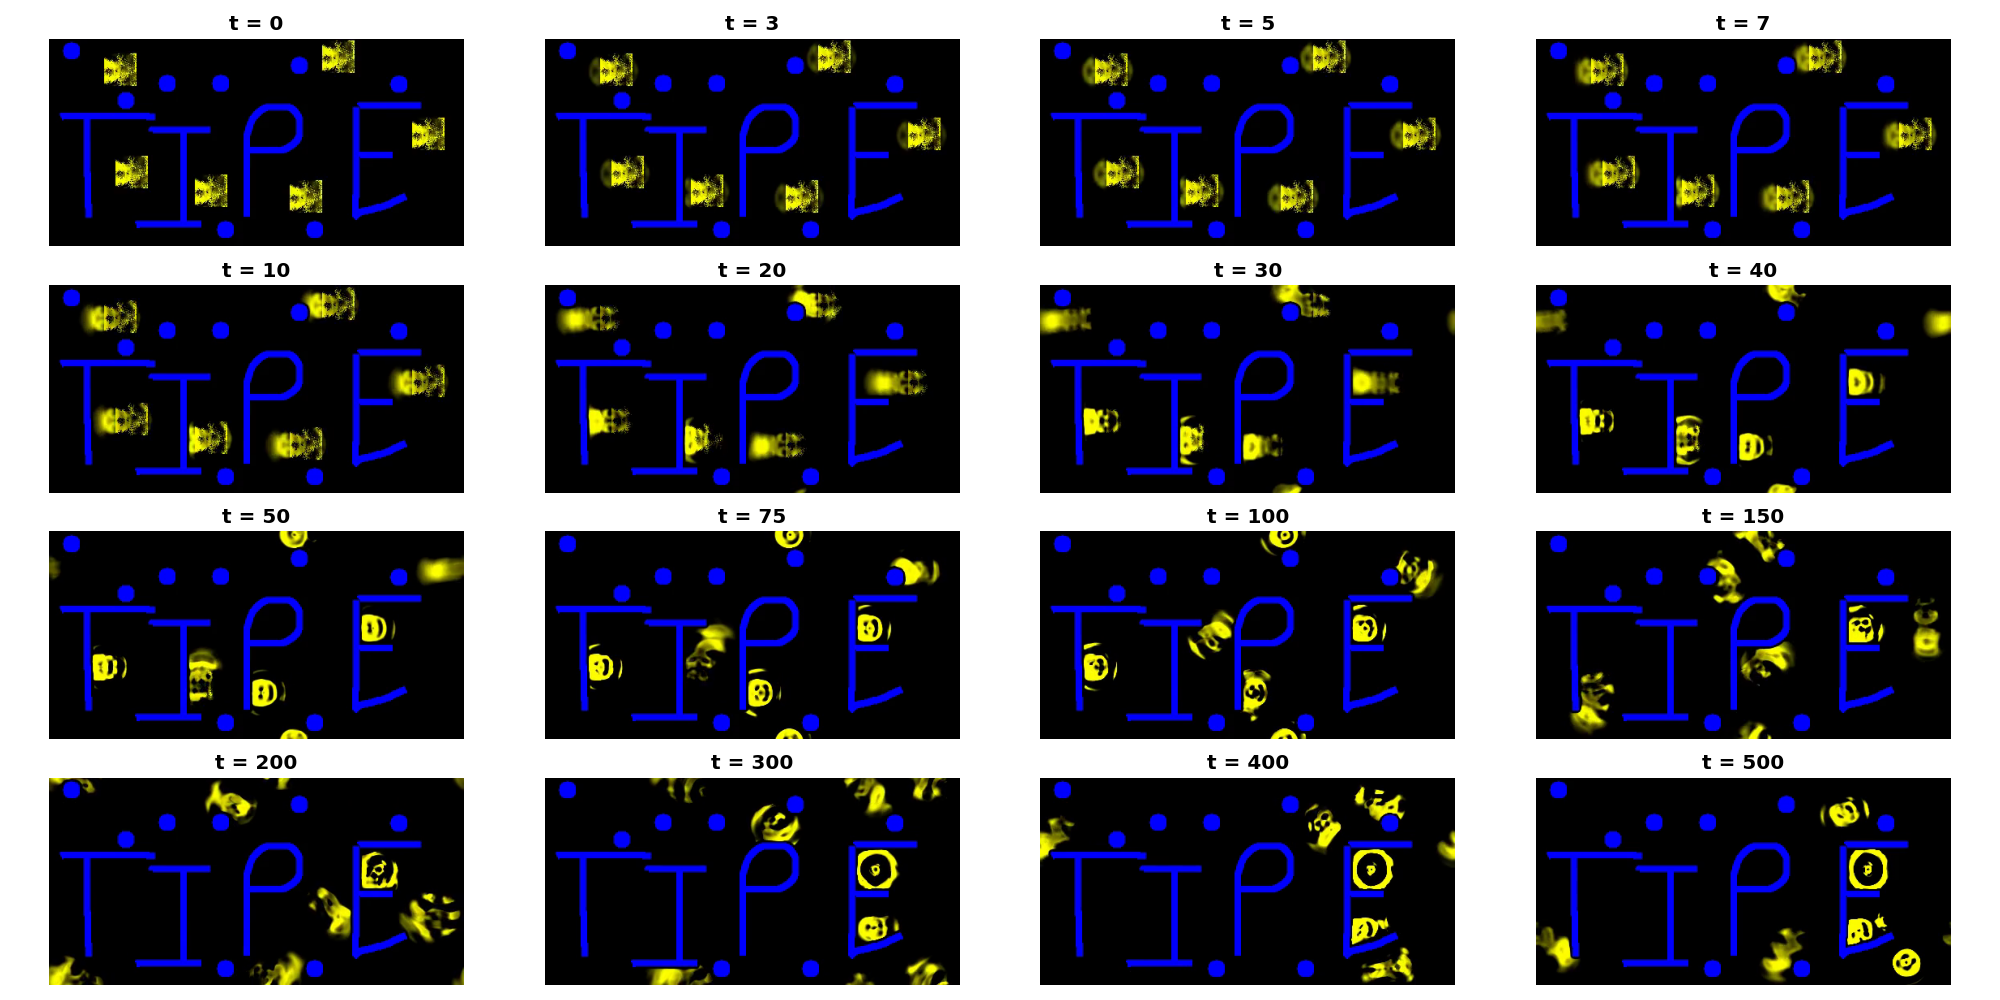
\includegraphics[width=\textwidth]{evolution_machine_learning.png}

		Observation de comportements \textbf{stables}, esp\`ece \textbf{en mouvement} qui \textbf{contourne des nouveaux obstacles}
	\end{center}

\end{frame}
\begin{frame}
    \frametitle{Objectifs}

    \begin{itemize}
        \item[\checkmark] \textbf{Généralisation} : du "Jeu de la Vie" à \textbf{Lenia}  
        \item[\checkmark] \textbf{Implémentation} de Lenia et de plusieurs de ses \textbf{extensions} en \textbf{python} \faPython
        \item[\checkmark] \textbf{Observation} d'automates aux \textbf{comportements macroscopiques remarquables}
        \item[$\sim$] Utilisation de méthodes d'\textbf{apprentissage automatique} dans l'exploration d'automates :
            \begin{itemize}
                \item[$\sim$] Implémentation de l'algorithme IMGEP
                \item[\checkmark] \textbf{Découverte} d'une nouvelle espèce remarquable
                \item[$\times$] Combinaison de plusieurs espèces aux différents comportements 
            \end{itemize}
    \end{itemize}

\end{frame}

\begin{frame}
	\frametitle{Annexe - Démonstration du théorème de convolution (1)}

	Soit $f, g$ deux fonctions réelles intégrables sur $\mathbb{R}$, on note
	\[
		y(x) = (f \star g)(x) = \int_{t = -\infty}^{+\infty} f(x-t)g(t)\,dt
	\]
	qui a pour transformée de Fourier :
	\[
		Y(\omega) = \mathbf{F}(y)(\omega) = \int_{x = -\infty}^{+\infty} \left[ \int_{t = -\infty}^{+\infty} f(x-t)g(t)\,dt \right] e^{-i\omega x}\,dx
	\]
	et donc en supposant l'interversion des intégrales licite :
	\[
		Y(\omega) = \int_{t = -\infty}^{+\infty} g(t)e^{-i\omega t} \left[ \int_{x = -\infty}^{+\infty} f(x-t) e^{-i\omega (x - t)}\,dx \right] \,dt
	\]
\end{frame}

\begin{frame}
	\frametitle{Annexe - Démonstration du théorème de convolution (2)}

	Et donc en effectuant le changement de variable affine $u = x - t$
	\begin{align*}
		Y(\omega) &= \int_{t = -\infty}^{+\infty} g(t)e^{-i\omega t} \left[ \int_{u = -\infty}^{+\infty} f(u) e^{-i\omega u}\,du \right] \,dt \\
		&= \left( \int_{t = -\infty}^{+\infty} g(t)e^{-i\omega t}\,dt \right) \left( \int_{u = -\infty}^{+\infty} f(u) e^{-i\omega u}\,du \right) \\
		&= \mathbf{F}(f)(\omega) \mathbf{F}(g)(\omega)
	\end{align*}
	D'où
	\[
		\mathbf{F}(f \star g) = \mathbf{F}(f)\mathbf{F}(g) 
	\]
\end{frame}

\begin{frame}
	\frametitle{Annexe - Illustrations de l'algorithme d'apprentissage (1)}
	
	\centering
	\begin{figure}[H]
		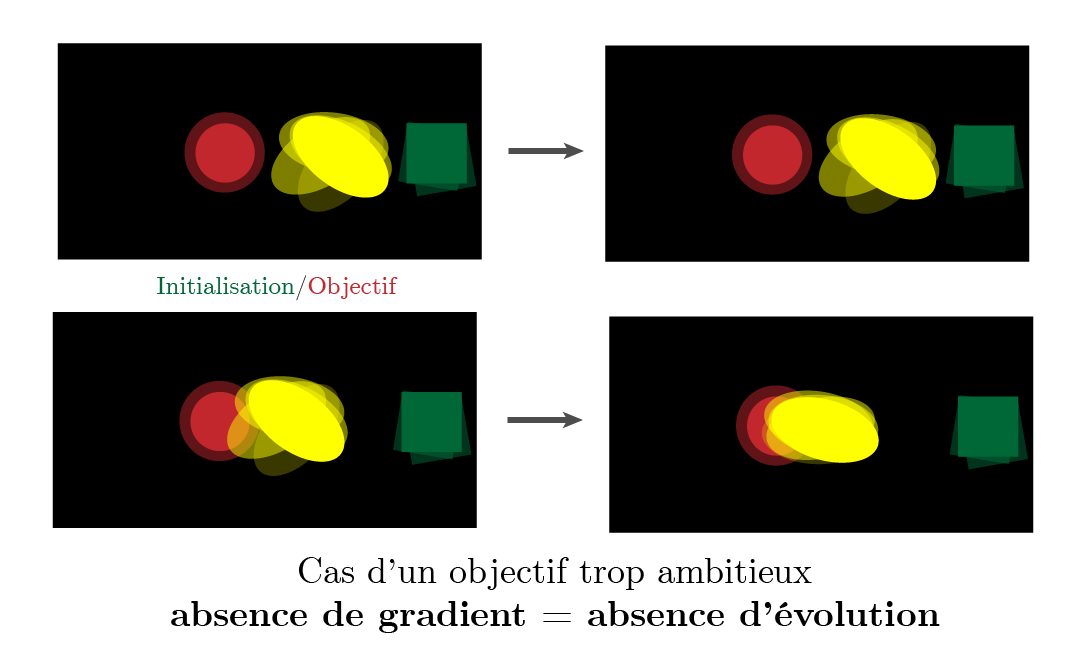
\includegraphics[width=.9\textwidth]{illustration_bad_target.png}
	\end{figure}
\end{frame}

\begin{frame}
	\frametitle{Annexe - Illustrations de l'algorithme d'apprentissage (2)}
	\begin{figure}[H]
		\centering
		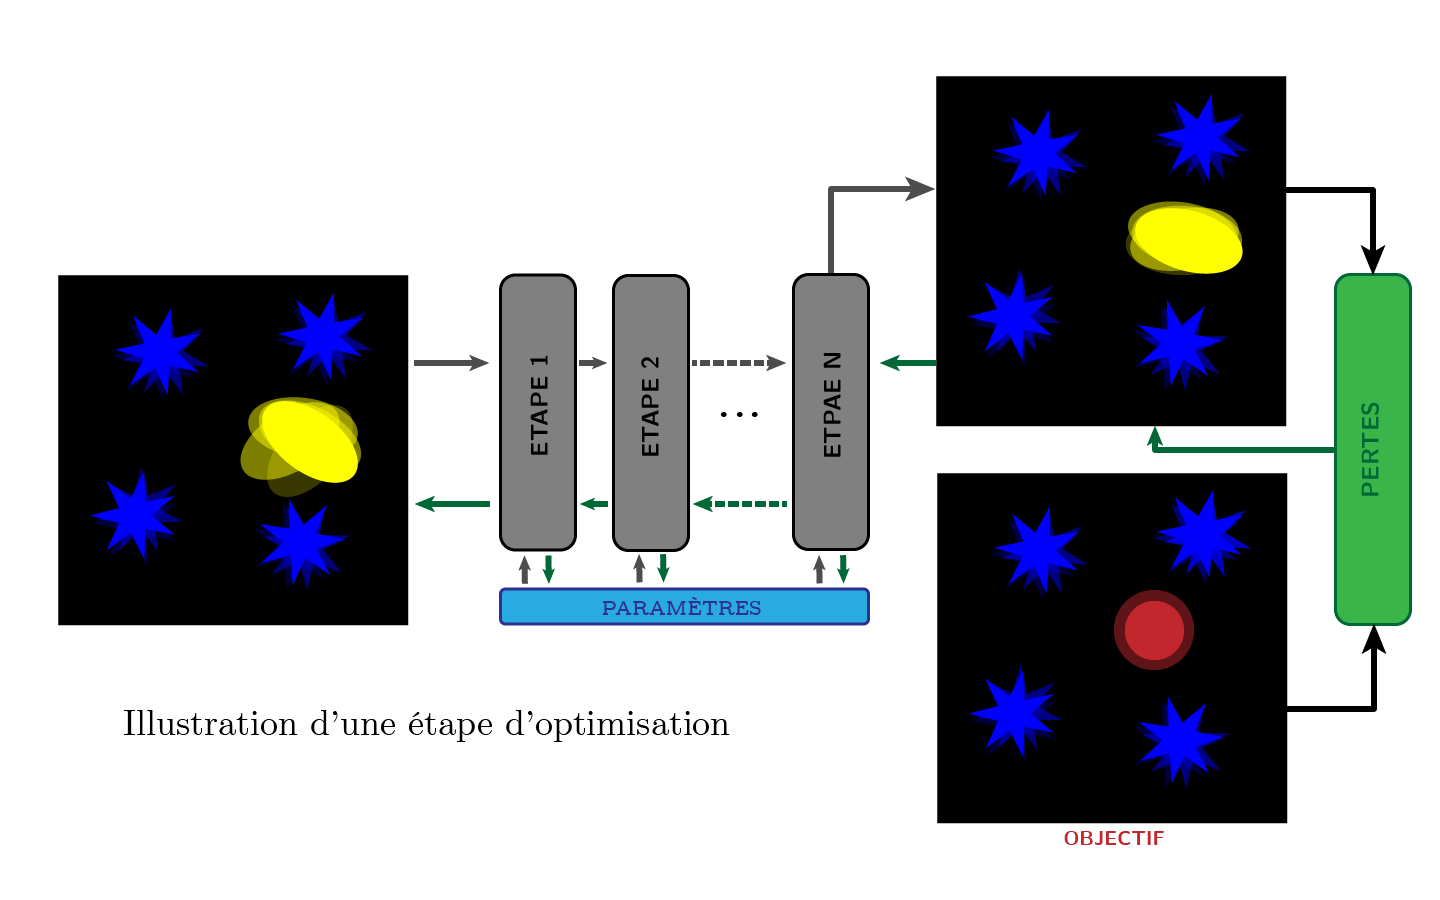
\includegraphics[width=\textwidth]{illustration_optimization_step.png}
	\end{figure}
\end{frame}

\begin{frame}
	\frametitle{Annexe - Transformation de Fourier Rapide}
	\begin{block}{FFT($x$):}
		\begin{algorithm}[H]
			$N \gets \text{longueur de } x$ \;
			\If{$N = 1$}{
				\Return $x$
			}
			$\omega \gets e^{-2\pi i / N}$ \;
			$x_{\text{pair}} \gets x[0], x[2], x[4], \ldots, x[N-2]$ \;
			$x_{\text{impair}} \gets x[1], x[3], x[5], \ldots, x[N-1]$ \;
			$X_{\text{pair}}, X_{\text{impair}} \gets \text{FFT}(x_{\text{pair}}), \text{FFT}(x_{\text{impair}})$ \;
			$X \gets [\;] * N$ \;
			\For{$k = 0$ to $N/2 - 1$}{
				$X[k] \gets X_{\text{pair}}[k] + \omega^k \cdot X_{\text{impair}}[k]$ \;
				$X[k + N/2] \gets X_{\text{pair}}[k] - \omega^k \cdot X_{\text{impair}}[k]$ \;
			}
			\Return $X$
		\end{algorithm}	
	\end{block}
\end{frame}

\begin{frame}
	\frametitle{Annexe - Complexités (temporelles)}
	
	Complexité d'une \textbf{évolution} Lenia de taille $n \times n$: $O(n^2 \log n)$ 
	\vfill

	Complexité d'une \textbf{éxécution} Lenia de $n_{\text{exec}}$ : $O(n_{\text{exec}}n^2 \log n)$
	\vfill

	Complexité d'une \textbf{étape IMGEP} : $O((n_{\text{opti}} + n_{\text{test}})n_{\text{exec}}n^2 \log n)$
	\vfill
	
	Complexité \textbf{totale} : $O(n_{\text{IMGEP}}(n_{\text{opti}} + n_{\text{test}})n_{\text{exec}}n^2 \log n)$
	\vfill

	\textbf{Temps d'exécution} de l'algorithme $\approx 25 \text{min}$ ($n_{\text{IMGEP}} = 160$, $n_{\text{opti}} = 15$, $n_{\text{test}} = 20$)
\end{frame}

\begin{frame}
	\frametitle{Annexe - Applications}
	
	\textbf{Biologie} : \begin{itemize}
		\item Motif de coquillages (\textit{cônes, cymbiolae})
		\item Comportement cellulaire (\textit{Firoblaste})
	\end{itemize}

	\textbf{Physique} : \begin{itemize}
		\item Propagation d'un feu de forêt
		\item Automate cellulaire stochastique -> étude statistique de matière condensée
	\end{itemize}

	\textbf{Chimie} : \begin{itemize}
		\item Oscillateur chimique (réaction(s) de \textit{Belooussov-Jabotinski})
	\end{itemize}

	\textbf{Autres} : \begin{itemize}
		\item Génération de labyrinthes
		\item Trafic routier
	\end{itemize}
\end{frame}
{
\setbeamercolor{background canvas}{bg=}
\foreach \n in{1,...,34}  {
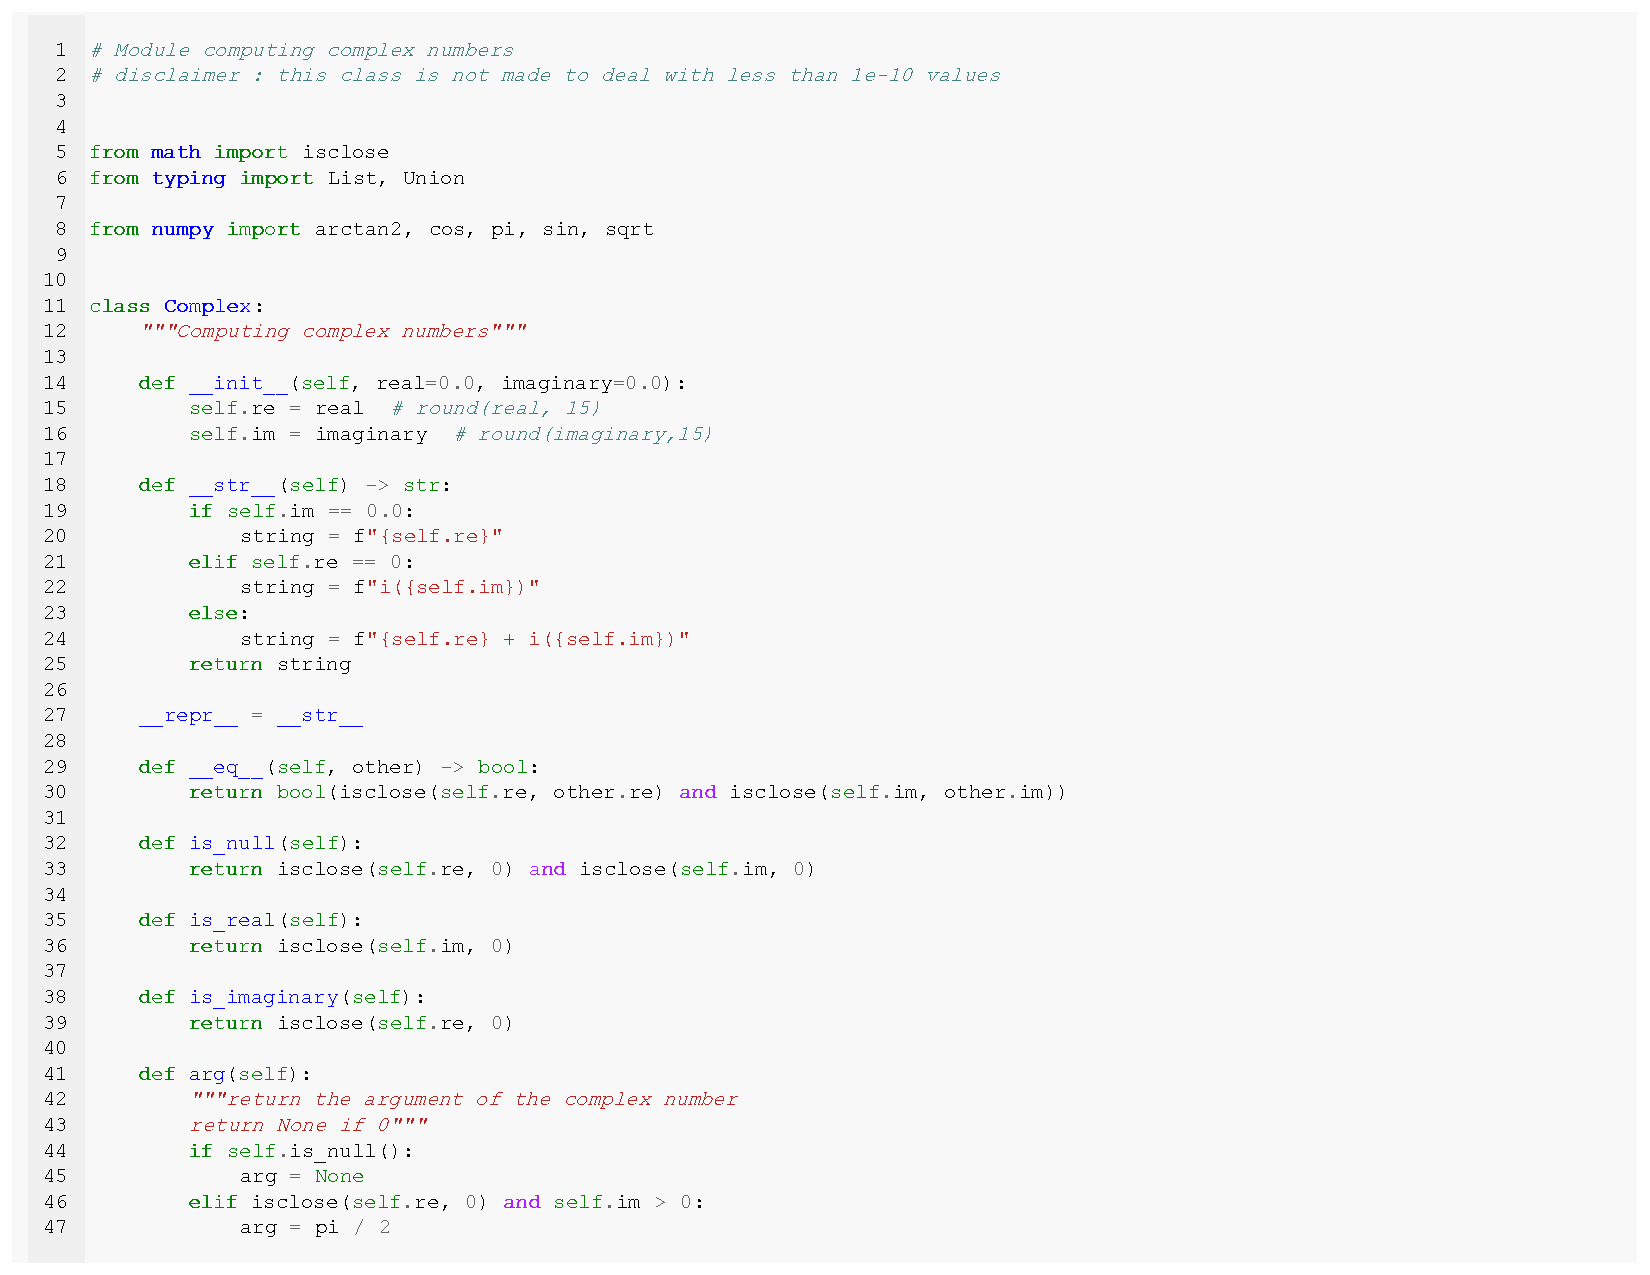
\includepdf[pages=\n]{img/all_code_merged_landscape.pdf}
}
}
\end{document}
